\section{Modelling of the Traction of the Metallic Strip}
As we said in the introduction, we know from a physical intuition that the traction in the metallic strip depends mainly on the difference of speed between the rolls, rather than on each of the speeds individually. For this reason, we only have to determine $G(p)$ as described in figure \ref{fig:tractionInput}, where $\omega_i$ is the speed of a motor, and $t$ is the traction of the metallic strip.
\begin{figure}[htbp]
\centering
\begin{tikzpicture}[auto, node distance=2cm,>=latex']
    % We start by placing the blocks
    \node [sum] (sum) {};
    \node [input, left of = sum, yshift = 1cm] (vr) {};
    \node [input, left of = sum, yshift = -1cm](vl) {};
    \node [sum, right of = sum, xshift = 1cm](addspeedsetpoint){};
    \node [input, below of = addspeedsetpoint](speed0){};
    \node [block, right of = addspeedsetpoint, xshift = 1cm](strip){$G(s)?$};
    \node [sum, right of = strip, xshift = 2cm](addtracsetpoint){};
    \node [input, below of = addtracsetpoint](tracsetpoint){};
    \node [output, right of = addtracsetpoint](trac){};

    % Once the nodes are placed, connecting them is easy.
    \draw [draw,->] (vr) node [yshift = 3mm]{$\omega_R$} -| node [pos = 0.9]{$+$} (sum);
    \draw [draw,->] (vl) node [yshift = 3mm]{$\omega_L$} -| node [pos = 0.9]{$-$} (sum);
    \draw [draw,->] (sum) -- node {$\Delta_\omega$} node[pos = 0.9]{$+$}  (addspeedsetpoint);
    \draw [draw,->] (speed0) -- node{${\Delta_\omega}_0$} node [pos = 0.9]{$-$} (addspeedsetpoint);
    \draw [draw,->]  (addspeedsetpoint) -- node{${\tilde{\Delta_\omega}}$} (strip);
    \draw [draw,->] (strip) -- node {$\tilde{f}$} node[pos = 0.9]{$+$} (addtracsetpoint);
    \draw [draw,->] (tracsetpoint) -- node {$f_0$} node[pos = 0.9]{$+$} (addtracsetpoint);
    \draw [draw,->] (addtracsetpoint) -- node {$f$} (trac);

\end{tikzpicture}
\caption{\label{fig:tractionInput}Simple gray-box model of the traction of the metallic strip}
\end{figure}

Furthermore, we also know that $G(s)$ should contain a close-to-perfect integrator. Indeed, if we increase $\Delta_\omega$ slightly from the setpoint ${\Delta_\omega}_0$, we expect the tension in the metallic strip to rise indefinitely until breakage. This is also confirmed by the experience: we observe that the system's response to a real world pulse is really close to a step, as showed in figure \ref{fig:tracImpulseResponse}.

\begin{figure}[htbp]
\centering
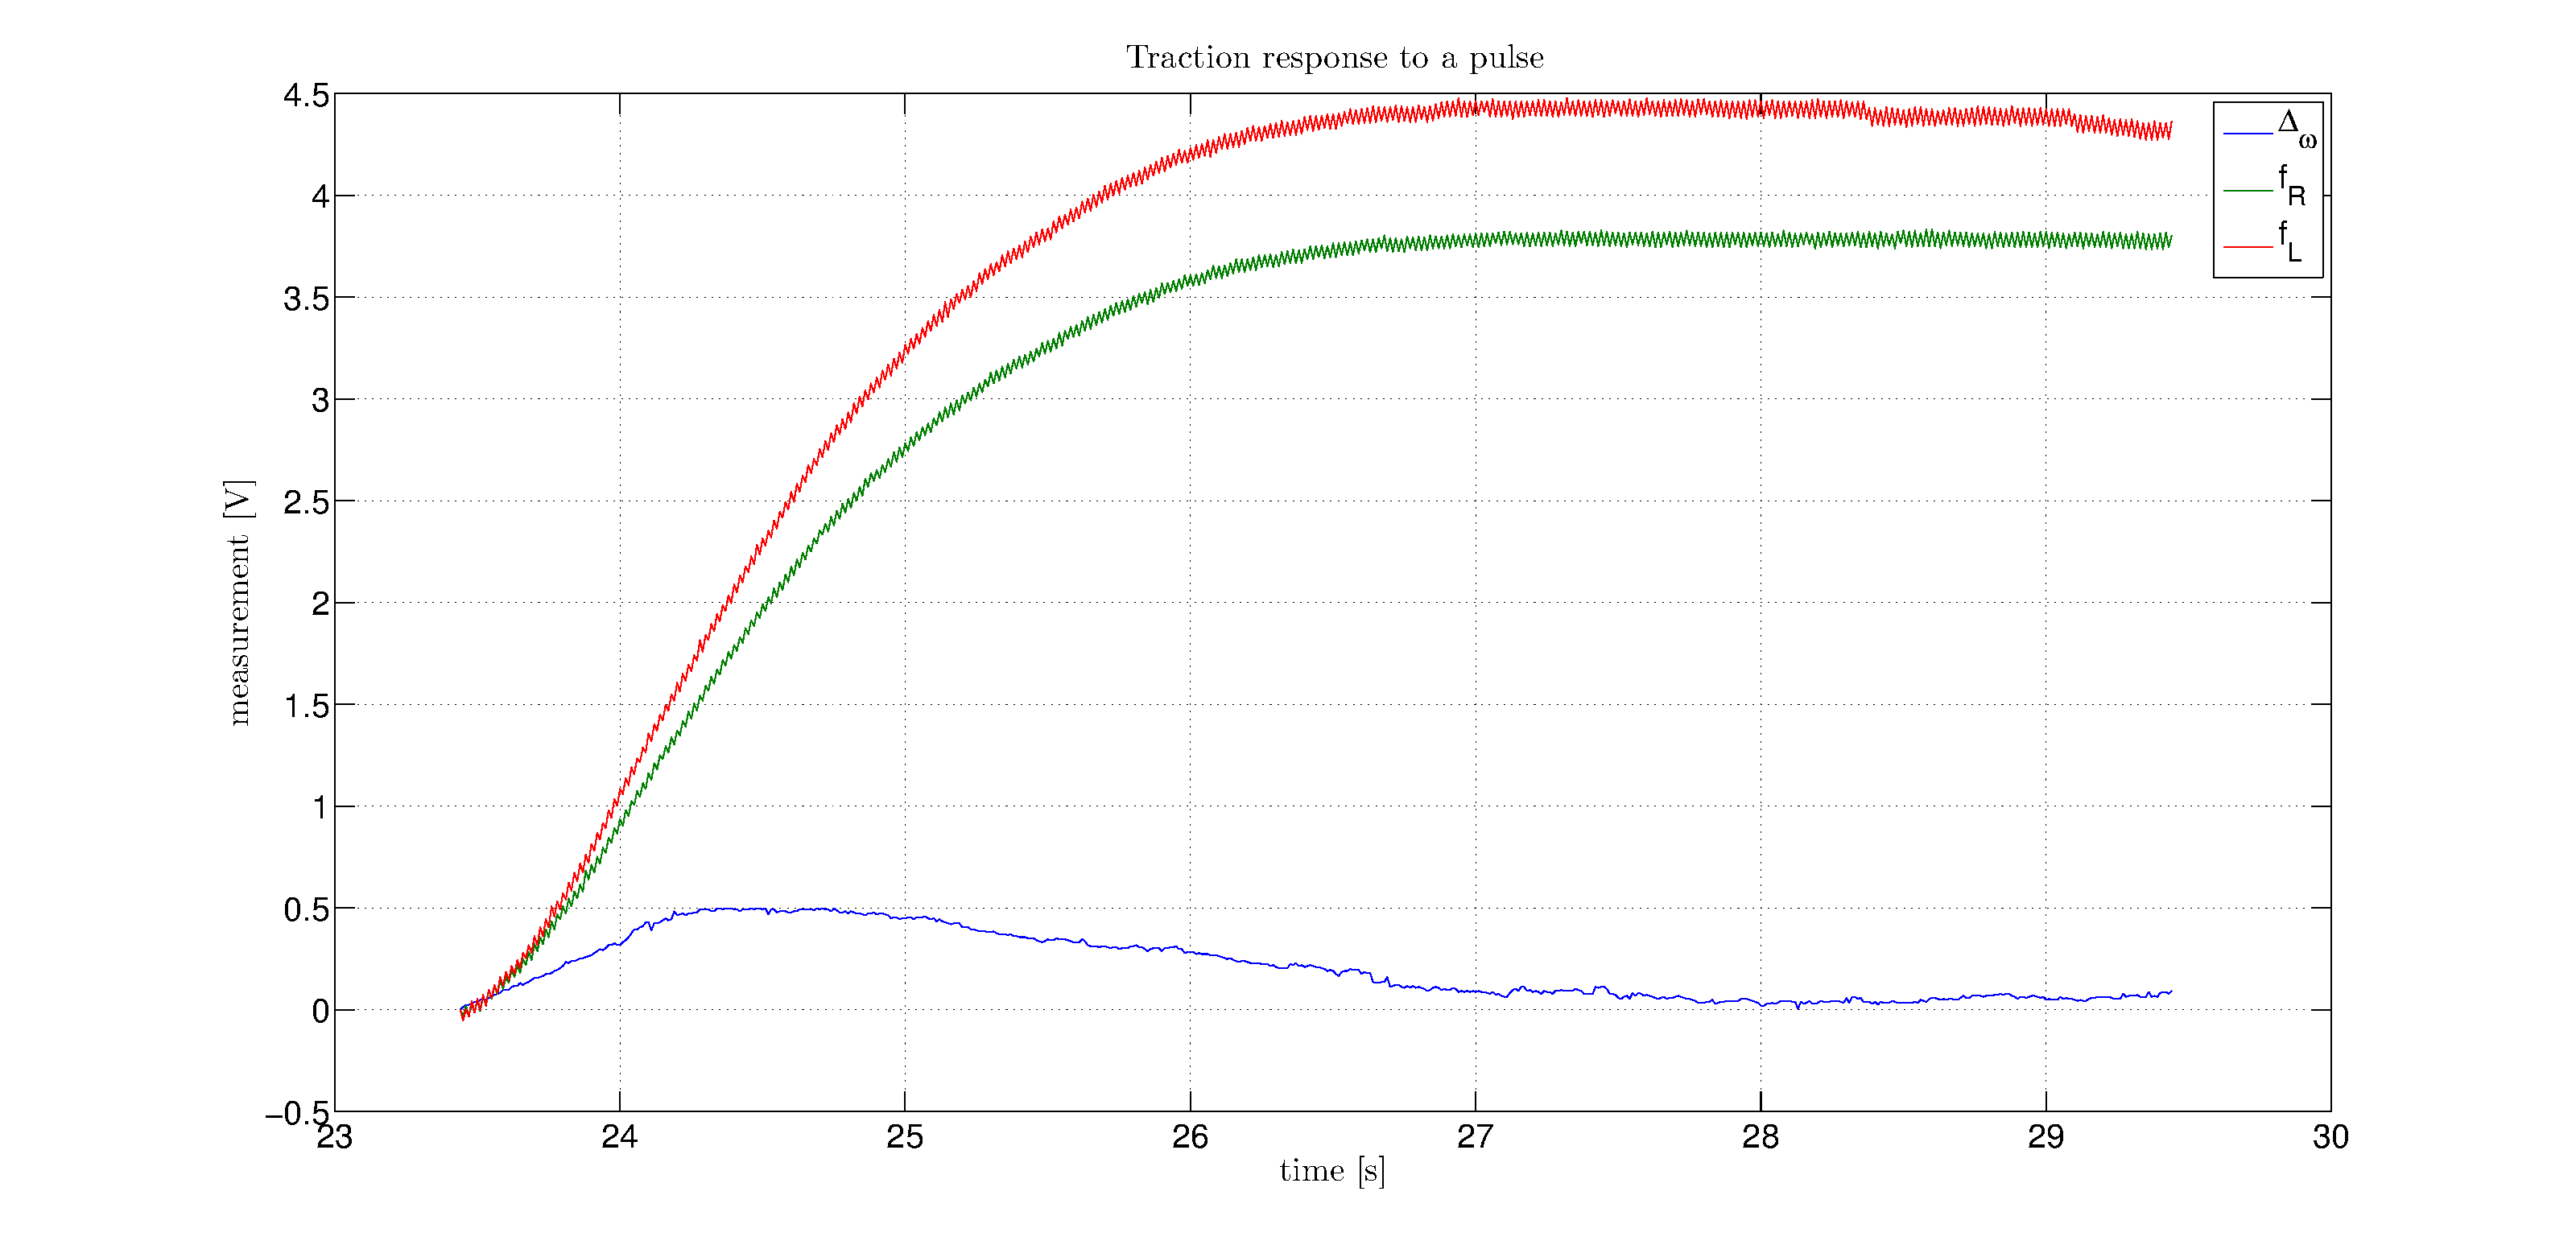
\includegraphics[width = \textwidth]{tractionPulse.pdf}
\caption{Traction response to a real world pulse\label{fig:tracImpulseResponse}}
\end{figure}

Finally, we also see that a second order numerical approximation of the dynamics always yields a pole that is very close to zero. However this leads the rest of the optimisation problem to be badly conditioned. This means that the second pole is not reliably placed, and that the final result does not fit the real response accurately. Moreover, a system with zero very far from the origin takes a really long time to simulate with simulink.

To solve this, we refine our gray-box approximation by introducing an integrator in the system, computing its response to $\tilde{\Delta_\omega}(t)$ and trying to determine the rest of the dynamics based on this new input and the observed response, as shown in figure \ref{fig:tractionGrayBox}, where $G(s) = \frac{1}{s}H(s)$.
\begin{figure}[htbp]
\centering
\begin{tikzpicture}[auto, node distance=2cm,>=latex']
    % We start by placing the blocks
    \node [input](input){};
    \node [square, right of = input, xshift = 1cm](integrator){$\frac{1}{s}$};
    \node [block, right of = integrator, xshift = 2.5cm](strip){$H(s)?$};
    \node [output, right of = strip](trac){};

    % Once the nodes are placed, connecting them is easy.
    \draw [draw,->]  (input) -- node{${\tilde{\Delta_\omega}}$} (integrator);
    \draw [draw,->]  (integrator) -- node{${\int^t_0\tilde{\Delta_\omega}}dt$} (strip);
    \draw [draw,->] (strip) -- node {$\tilde{f}$} (trac);
\end{tikzpicture}
\caption{\label{fig:tractionInput}Gray-box model of the traction of the metallic strip\label{fig:tractionGrayBox}}
\end{figure}

Fitting a simple first order transfer function to $H(s)$ is not easy because the dynamics between $\frac{\tilde{\Delta_\omega}(s)}{s}$ and $F_R(s)$ is very fast, as shown in figure \ref{fig:tractionPulseStep}. This leads to very large poles which are not well approximated and difficult to simulate, as previously stated.
\begin{figure}[htbp]
\centering
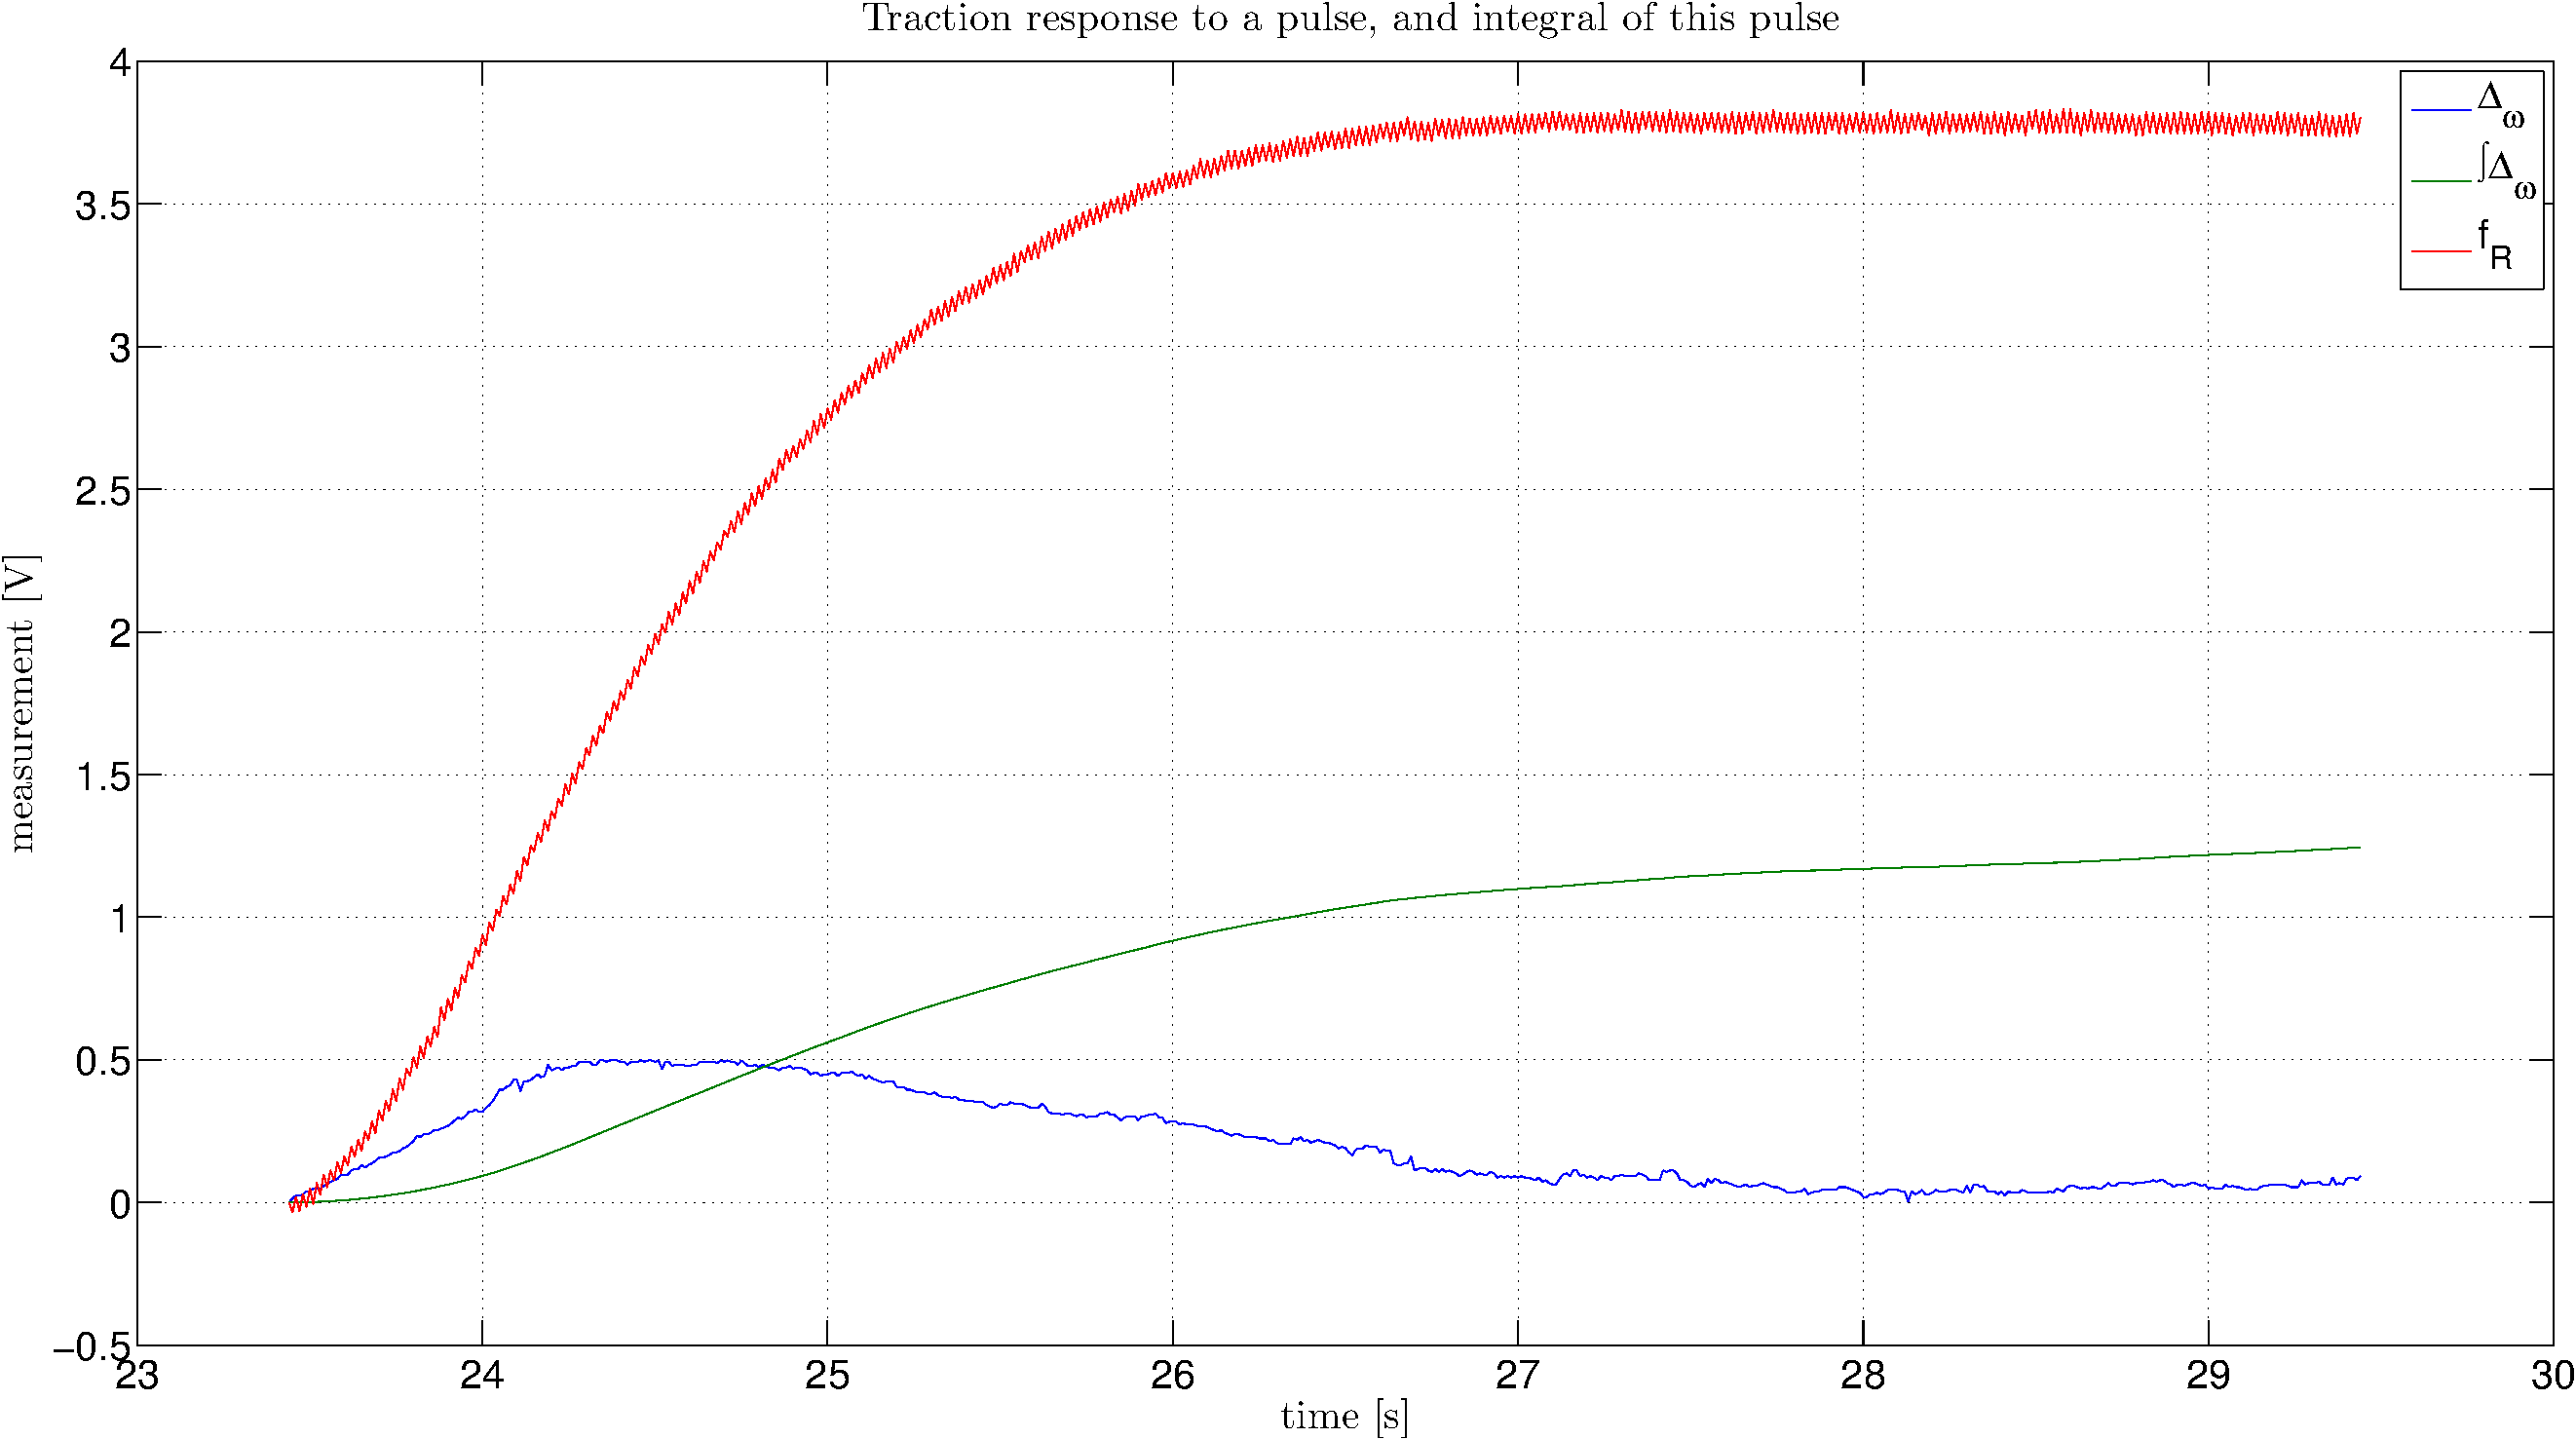
\includegraphics[width = \textwidth]{tractionPulseStep.pdf}
\caption{Right traction response to a pulse and output of the intermediate integrator\label{fig:tractionPulseStep}}
\end{figure}

To solve this, we tried to fit $H(s)$ with a transfer function of the form $K\frac{s-z_0}{s-p_0}$, because the introduction of a zero speeds up a step response, which would bring $p_0$ reasonably closer to the origin. The result is shown in figure \ref{fig:tracFit}, where we see that the following transfer function seems to fit the experience very well.
\[H(s) = 13.096\frac{s+0.9221}{s(s+4.063)}\]
\begin{figure}[htbp]
\centering
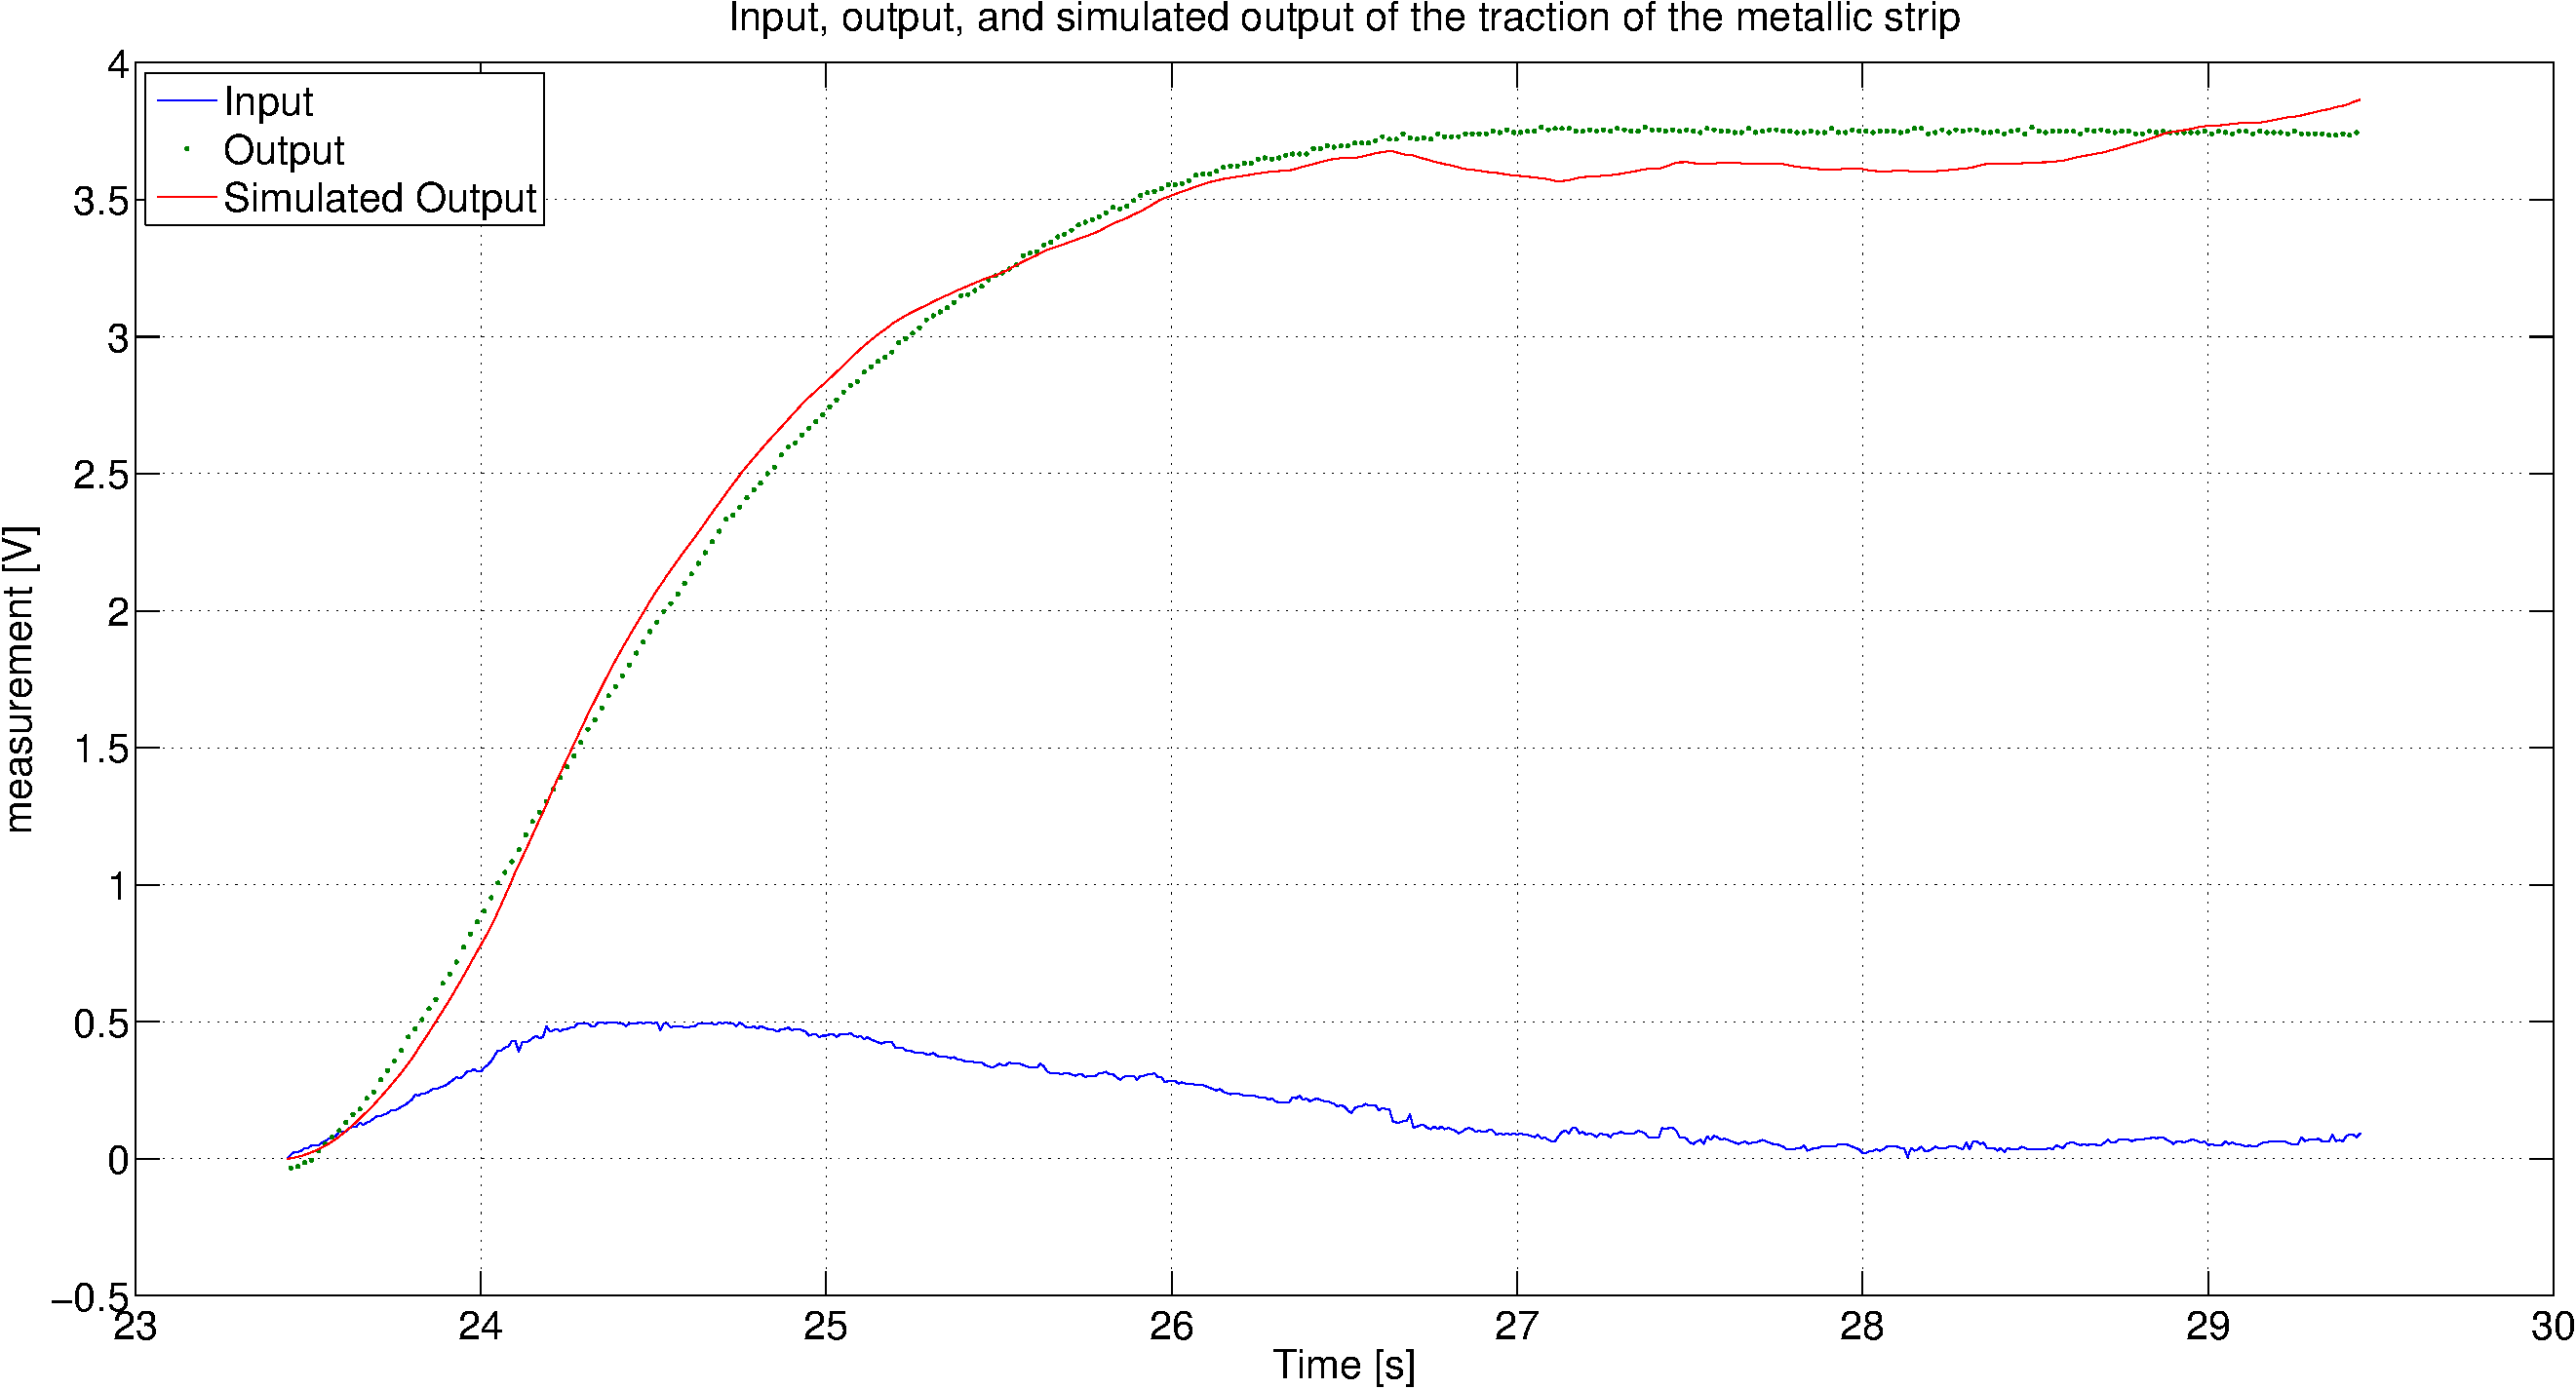
\includegraphics[width = \textwidth]{tracFit.pdf}
\caption{Input, output, and simulated output of the traction of the metallic strip\label{fig:tracFit}}
\end{figure}

